\lab{Linear Systems}{Linear Systems}
\objective{The fundamental problem of linear algebra is solving the linear system $A\x = \b$, if it is even possible.
There are many approaches to solving this problem, each with different problems and advantages.
In this lab we implement the LU Decomposition and introduce the SciPy library for linear algebra and sparse matrices.
}

\section*{Row Operations} % ---------------------------------------------------

When you perform a row operation on a matrix, you are really left-multiplying by some elementary matrix.
However, matrix multiplication is not the most efficient way to implement row operations. It is much faster to perform row operations by modifying the array in place, and only changing those entries that are affected by the operation.
The following code implements the three elementary row operations by modifying the array in place.

\begin{lstlisting}
def type_I(A, i, j):
    """Swap the i-th and j-th rows of A."""
    A[i], A[j] = np.copy(A[j]), np.copy(A[i])

def type_II(A, i, alpha):
    """Multiply the i-th row of A by a constant."""
    A[i] *= alpha

def type_III(A, i, j, alpha):
    """Add a constant multiple of the j-th row of A to the i-th row."""
    A[i] += alpha * A[j]
\end{lstlisting}

\subsection*{Programming Row Reduction} % -------------------------------------

Reduce a system to row echelon form (REF)\footnote{We do not require leading coefficients to be 1 in the REF.}, then use back system to the system by row reduction.

\begin{lstlisting}
>>> A = np.array([[4., 5., 6., 3.],[2., 4., 6., 4.],[7., 8., 0., 5.]])
>>> A
array([[ 4.,  5.,  6.,  3.],
       [ 2.,  4.,  6.,  4.],
       [ 7.,  8.,  0.,  5.]])
>>> type_III(A, 1, 0, A[1,0]/A[0,0])
>>> type_III(A, 2, 0, A[2,0]/A[0,0])
>>> type_III(A, 2, 1, A[2,1]/A[1,1])

>>> A
array([[ 4. ,  5. ,  6. ,  3. ],
       [ 0. ,  1.5,  3. ,  2.5],
       [ 0. ,  0. , -9. ,  1. ]])
\end{lstlisting}

The third row operation really only modifies a part of the third row because the first values in each affected row are each 0.
Modifying only those entries of the array that are affected by a row operation will save a lot of time when row reducing a large matrix.

Beware that round-off error in row reduction can cause serious problems.
Suppose we wish to row reduce a matrix $A$ as follows.

\begin{lstlisting}
>>> A = np.array([[4., 5., 6., 3.],[2., 2.5, 6., 4.],[7., 8., 0., 5.]])
array([[ 4.,  5.,  6.,  3.],
       [ 2.,  2.5,  6.,  4.],
       [ 7.,  8.,  0.,  5.]])
>>> A[1] -= (A[1,0]/A[0,0]) * A[0]
>>> A[2] -= (A[2,0]/A[0,0]) * A[0]
\end{lstlisting}

If we work this out by hand, at this point we have

\begin{align}
A = \left[\begin{array}{cccc}
4 &    5 &     6 &    3 \\
0 &    0 &     3 &  2.5 \\
0 & -7.5 & -10.5 & -.25
\end{array}\right].
\label{equ:row-reduction-no-errors}
\end{align}

If we swap the second and third rows, then the matrix is in row echelon form.
However, suppose that due to round-off error, the machine instead computes

\begin{align*}
A = \left[\begin{array}{cccc}
4 & 5        &     6 &    3 \\
0 & 10^{-15} &     3 &  2.5 \\
0 & -7.5     & -10.5 & -.25
\end{array}\right].
\end{align*}

The algorithm would then attempt to pivot on the \li{A[1,1]} entry as follows.

\begin{lstlisting}
>>> A[2,1:] -= (A[2,1]/A[1,1]) * A[1,1:]
>>> A
array([[ 4. ,  5.0e+00 , 6.00e+00 ,  3.000e-00 ],
       [ 0. ,  1.0e-14 , 3.00e+00 ,  2.500e-00 ],
       [ 0. ,  0.0e+00 , 2.25e+14 ,  1.875e+14 ]])
\end{lstlisting}

The round-off error in the \li{A[1,1]} entry has affected the third row, and the matrix is now much different than the correct answer in (\ref{equ:row-reduction-no-errors}).
In larger matrices, round-off error can propagate through many steps in a calculation, resulting in garbage output.

Some of NumPy's matrix algorithms use row reduction.
NumPy's methods use several clever tricks to minimize the impact of round-off errors.
However, these methods may still give you garbage output due to round-off error, especially if the matrix is \emph{ill-conditioned}.
You should always be aware of this possibility.

\begin{problem}
\label{prob:REF}
Write a function which reduces a square matrix to REF.
You may make the following assumptions:
\begin{enumerate}
\item The matrix is invertible.
\item During your row reduction, a zero will never appear on the main diagonal.
\item All round-off errors may be ignored.
\end{enumerate}
During a row operation, do not modify any entries that you know will be zero before and after the operation.
\end{problem}

\subsection*{The LU Decomposition} % ------------------------------------------

The LU decomposition of a square matrix $A$ is a factorization $A=LU$ where $U$ is an upper triangular and $L$ is a lower triangular matrix.
In fact, $U$ is the REF of $A$ and $L$ is a product of Type III elementary matrices whose inverses reduce $A$ to $U$.
Thus, the LU decomposition is a way of storing the REF and ``how we got there.''

The LU factorization of $A$ exists only when $A$ can be reduced to REF using only Type III elementary matrices (no row swaps).
However, we can always permute the rows of $A$ to obtain a matrix that has an LU decomposition.
If $P$ encodes the row swaps, then a decomposition $PA = LU$ always exists.

If $A$ has an LU decomposition (not requiring row swaps), then we can find it as follows.
Reduce $A$ to REF with $k$ row operations, corresponding to matrices $E_1, \ldots, E_k$.
Then $U = E_k \ldots E_2E_1A,$ where $U$ is the REF of $A$.
Because there were no row swaps, each $E_i$ is a lower triangular Type III matrix. Then $E_i^{-1}$ is also lower triangular.
Thus, $L=(E_k \ldots E_2E_1)^{-1}$ is lower triangular, and $LU=A.$

Because $L=(E_k \ldots E_2E_1)^{-1} = IE_1^{-1}E_2^{-1}\ldots E_k^{-1}$, we can compute $L$ by right-multiplying the identity by the matrices we used to reduce $U$.
In fact, in this special situation, each right-multiplication will change only one entry of $L$.
We have the following algorithm for the LU decomposition, assuming it exists.

%
%\begin{itemize}
%\item Make a copy, $U$, of $A$.
%\item Make an identity matrix $L$ that is the same shape as $A$.
%\item Iterate through the entries below the diagonal of $U$.
%
%Now for each entry below the main diagonal of $U$ do the following:
%   \begin{itemize}
%   \item Set the corresponding entry of $L$ to the quotient of the current entry of $U$ and the entry of the main diagonal of $U$ located above the current entry.
%   \item Perform the type 3 row operation to set the current entry of $U$ to 0.
%       Do not modify any entries known to be 0.
%   \end{itemize}
%\item Return $L$ and $U$
%\end{itemize}

\begin{algorithm}
\begin{algorithmic}[1]
\Procedure{LU Decomposition}{$A$}
\State Store the dimensions $(m, n)$ of $A$
\State Initialize the $U$ matrix as a copy of $A$
\State Initialize the $L$ matrix as the $n\times n$ identity matrix
\State Then create your matrices as follows:
\For{$j=0 \ldots n-1$}
    \For{$i=j+1 \ldots m-1$}
    %\State $L[i,j] \gets U[i, j]/U[j, j]
    \State Set each element of $L$ to the corresponding element of $U$ divided by $U[j,j]$
    %\State $U[i,j:] \gets U[i,j:] - L[i,j]U[j, j:]$
    \State Set $U[i,j:]$ to itself minus $L[i,j] \times U[j,j:]$
    \EndFor
\EndFor
\State \pseudoli{return} $L, U$
\EndProcedure
\end{algorithmic}
\caption{The algorithm for the LU decomposition of a matrix $A$. This algorithm returns lower triangular $L$ and upper triangular $U$ such that $A = LU$.}
\label{Alg:gram_schmidt}
\end{algorithm}

\begin{problem}
\label{prob:LU_copy}
Write a function that finds the LU decomposition of a square matrix.
You may assume that the matrix has an LU decomposition.
\end{problem}

The LU decomposition can be performed in-place by storing $U$ on and above the main diagonal of the array and storing $L$ below it.
The main diagonal of $L$ does not need to be stored since all its entries are ones.

\begin{problem}
Modify your solution to Problem \ref{prob:LU_copy} so that the function computes the LU decomposition in place.
\end{problem}

\subsection*{Applications of the LU decomposition} % --------------------------

The LU decomposition is a more efficient way to solve linear systems than row reduction, and it can also be used to quickly compute inverses and determinants.
SciPy implements these methods in the \li{linalg} module, specifically in the functions \li{la.lu_factor()}, \li{la.solve()}, \li{la.inv()}, and \li{la.det()}.

Let us see how to use the LU decomposition to solve matrix equations.
Suppose that after row swaps, $A$ has the decomposition $PA = LU$.
Then $Ax=b$ is equivalent to $LUx=Pb$.
We can solve this system by first solving $Ly = Pb$ and then $Ux = y$.
Since $L$ and $U$ are triangular, these systems can be solved with backward and forward substitution, which is faster than row reduction.
Thus, we can perform row reduction once to compute the $LU$ factorization of $A$, and then we can use substitution to solve $Ax=b$ for many different values of $b$.
This technique is significantly faster than storing $A^{-1}$ and then computing $A^{-1}b$ (see Problem \ref{prob:solve}).

\begin{problem}\label{prob:solve}
In this problem you will solve the system $Ax = b$ for fixed $A$ and many different values of $b$.
You will do this in two ways.
For a random $1000 \times 1000$ array $A$ and a random $1000 \times 500$ array $B$ do the following.
\begin{enumerate}
\item Time \li{la.lu_factor(A)}.
\item Time \li{la.inv(A)}.
\item Store the output of \li{la.lu_factor()}. Time \li{la.lu_solve()} on this stored output and $B$.
\item Store the inverse of $A$. Time how long it takes to multiply $A^{-1}$ by $B$.
\item What can you conclude about the more efficient way to solve linear systems?
\end{enumerate}
\end{problem}

Our technique for solving linear equations can also be used to invert matrices.
We can compute $A^{-1}$ by solving $LUx_i = P_i$ for every $P_i$ that is a column of $P$.
Then $A^{-1}$ is the matrix with columns $x_1, x_2, \ldots, x_n$.

Finally, the LU decomposition also gives us an efficient way to compute determinants.
If $PA=LU$, then $\det(A) = [\det(P)]^{-1}\det(L)\det(U)$.
But the determinant of a triangular matrix is the product of its diagonal entries, and every diagonal entry of $L$ is 1.
Also, $\det(P)$ is the number of row swaps we applied to $A$ to put it in the appropriate form.
So if $U$ has diagonal entries $u_{ii}$ for $i=1, \ldots, n$, then

\[
\det(A) = (-1)^S\left(\displaystyle\prod_{i=1}^nu_{ii}\right),
\]

where $S$ is the number of row-swaps.

%\begin{problem}
%\label{prob:lusolve}
%Write a function that takes the LU decomposition computed by the second function you made in Problem \ref{prob:LU} and another array representing the right hand side of a linear system and modifies the second array in place so that it represents the solution to the linear system.
%No changes to the array storing the LU decomposition are necessary.
%\end{problem}
%

\begin{problem}
\label{prob:det}
Write a function that finds the determinant of a matrix using \li{la.lu_factor()} and the algorithm described above.
Read the documentation to learn about the output of \li{la.lu_factor()}.
Hint: If the $i^{th}$ entry of the output \li{piv} does not equal $i$, this means that a row swap occurred.
\end{problem}

\section*{SciPy} % ============================================================

SciPy is . . .

\subsection*{Linear Algebra} % ------------------------------------------------

Both NumPy and SciPy have a linear algebra library, but the SciPy library is larger.
The SciPy linear algebra library is typically imported as follows:

\begin{lstlisting}
from scipy import linalg as la
\end{lstlisting}

The linear algebra library contains several functions to construct special
matrices, located in \li{linalg.special_matrices}.
There are also functions that will invert matrices, find determinants and norms, solve linear systems and least squares problems, and find special matrix decompositions.
You can read more about the linear algebra capabilities of SciPy in the documentation for the \li{linalg} module found at \url{http://docs.scipy.org/doc/scipy/reference/linalg.html}.

Finally, the \li{scipy.linalg} library has a \li{matrix} class that is very
similar to a 2-D NumPy array.
The matrix class can be convenient when doing matrix operations.
However, in such situations we still recommend using NumPy arrrays, which have many of the same features and are also compatible with all other SciPy operations.

The \li{scipy.linalg} library will be essential for the remainder of the labs in this manual.

\subsection*{Spatial Complexity} % --------------------------------------------

Analogous to temporal complexity, the spatial complexity of an algorithm is a function that describes how the algorithm's memory use increases as input sizes to the algorithm increase. For example, if your algorithm needs to store an $n \times n$ matrix, its memory use will increase at least as fast as $n^2$. Spatial complexity is important because  the spatial complexity of an algorithm can affect its speed in several ways. The most important way is that when the memory usage exceeds the amount of available RAM, the machine must use either the hard disk or some other slower method of storage.

This vocabulary allows us to discuss the question at the start of this lab: ``How long will a computer take to execute this algorithm?" The amount of time a computer takes to execute an algorithm depends both on the algorithm's temporal complexity and on its spatial complexity.

\begin{comment}
\begin{problem}\label{prob:complexity_problem}
In this problem you will analyze the complexity of the following functions:

\begin{lstlisting}
# Run through a single for loop.
def func1(n):
    n = 500*n
    sum(xrange(n))
# Run through a double for loop.
def func2(n):
    n = 3*n
    t = 0
    for i in xrange(n):
        for j in xrange(i):
            t += j
# Square a matrix.
def func3(n):
    n = int(1.2*n)
    A = np.random.rand(n, n)
    np.power(A, 2)
# Invert a matrix.
from scipy import linalg as la
def func4(n):
    A = np.random.rand(n, n)
    la.inv(A)
# Find the determinant of a matrix.
from scipy import linalg as la
def func5(n):
    n = int(1.25*n)
    A = np.random.rand(n, n)
    la.det(A)
\end{lstlisting}

Plot your results in the following manner:
\begin{enumerate}
\item Time how long each function takes to run on an input of size $n$ for $n=100, 200, 400$, and $800$.
\item For each function, plot a line using $100, 200, 400$, and $800$ for the $x$-values and your runtimes for the $y$-values. Make sure your $y$-values are all in the same units! When you call the matplotlib function \li{plot}, specify a value for the keyword parameter \li{label} so that you can reference each line later. For example, the call \li{plt.plot(x, y, label='Function 1')} attaches the label ``Function 1" to the line made by \li{x} and \li{y}.
\item After plotting all your lines, call the function \li{legend} to draw a legend on your graph. Use the keyword argument \li{loc} to specify the location of the legend. Some possible values are \li{'upper left'} and \li{'right'}. See the documentation for more options. Your final graph should look something like the figure below.\footnote{From this graph, you can see that inverting a matrix is an incredibly time-consuming operation. In Lab \ref{lab:ChangeBasis} you will learn fast algorithms for solving linear systems without inverting matrices. In fact, inverting matrices is so costly in terms of temporal and spatial complexity that there is hardly ever a good reason to do it.}
\end{enumerate}
Note that we rescaled the inputs to the functions so that your lines would begin at roughly the same place on the y-axis.

\centering
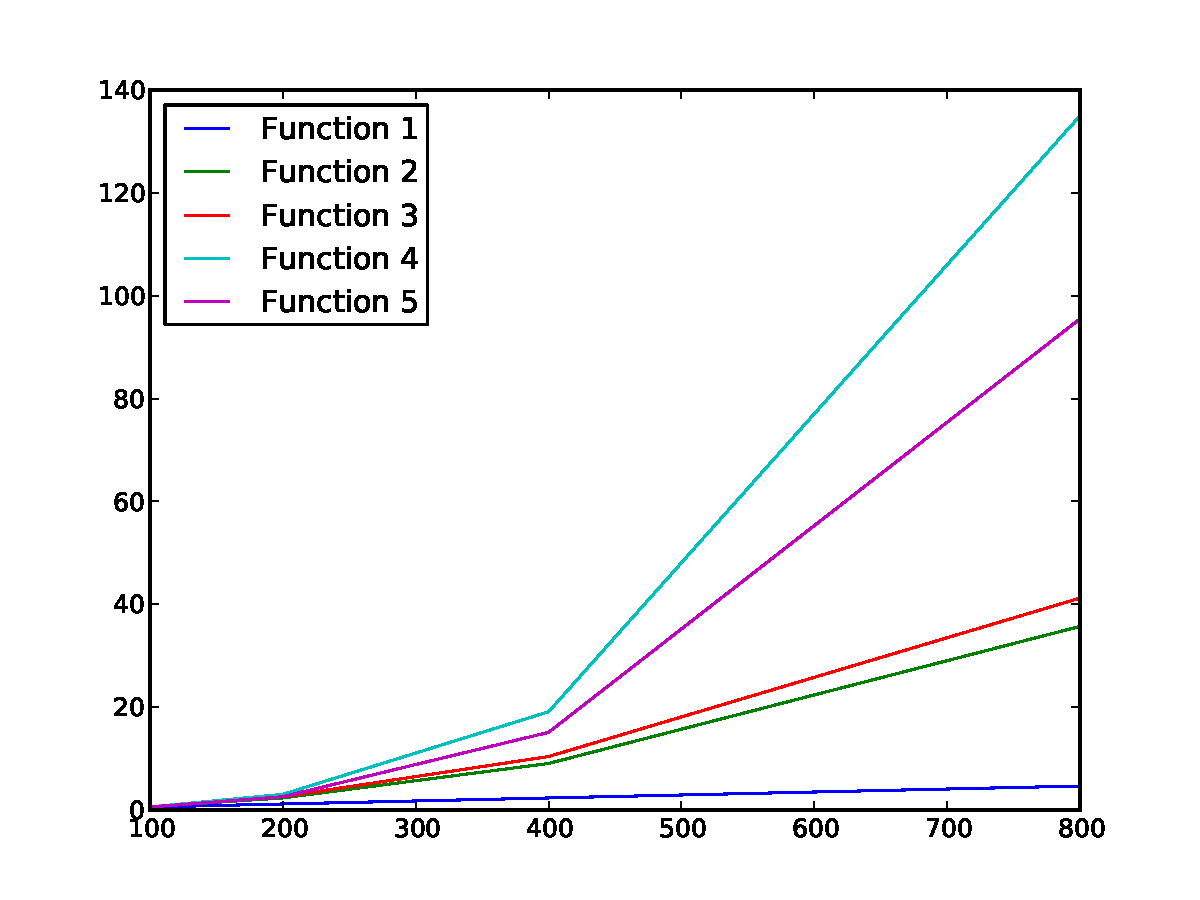
\includegraphics[width=\textwidth]{complexity_problem.pdf}

\end{problem}
\end{comment}

\section*{Sparse Matrices} % ==================================================

A matrix with relatively few nonzero elements is called \emph{sparse}.
Sparse matrices arise frequently in both theoretical and real-world applications.
We can take advantage of the sparse structure of these matrices to use less memory and decrease computation time.

For example, diagonal matrices are sparse.
Storing an $n \times n$ diagonal matrix in the naive way means storing $n^2$ values in memory.
For most applications, it makes more sense to store the diagonal entries in a 1-dimensional array of $n$ values.
In addition to using less storage space, this allows for much faster matrix operations.
Using the standard algorithm to multiply a matrix by a diagonal matrix involves $n^3$ steps, but most of these are multiplying by or adding zero.
A smarter algorithm that knows all off-diagonal entries are zero can accomplish the same task much faster.

\subsection*{The Sparse Module} % ---------------------------------------------

The SciPy module \li{sparse} has storage methods to reduce the temporal and spatial complexity of handling sparse matrices.
When we are not using these special methods, we say we are storing the \emph{full} matrix.
We can also use \li{sparse} methods on dense matrices (matrices with mostly nonzero entries), but doing so will take longer than using the usual methods for handling full matrices.

The difference in spatial complexity occurs because a full array occupies a block of memory for each entry, so an $n \times n$ array requires $n^2$ blocks of memory.
By contrast, SciPy's \li{sparse} methods store only the nonzero entries and their locations in the array.
As long as most entries are 0 (i.e., the matrix is sparse), this decreases spatial complexity.
You minimize spatial complexity when you store a sparse matrix with the \li{sparse} module and a dense matrix as a full (or ``regular'') matrix.

SciPy has seven sparse matrix types, listed in Table \ref{table:smr}.
Each type is optimized either for storing sparse matrices whose nonzero entries follow certain patterns, or for performing certain computations.
For example, the \li{csc_matrix} and \li{csr_matrix} types are optimized for arithmetic operations.
We will introduce some other types later in this lab. For more information, see the documentation (\url{http://docs.scipy.org/doc/scipy/reference/sparse.html}).

\begin{table}
\centering
\begin{tabular}{|r|l|}
\hline
Sparse Matrix Type & Description \\
\hline
\li{bsr_matrix} & Compressed Block Sparse Row\\
\li{coo_matrix} & Coordinate\\
\li{csc_matrix} & Compressed Sparse Column\\
\li{csr_matrix} & Compressed Sparse Row\\
\li{dia_matrix} & Sparse Diagonal\\
\li{dok_matrix} & Dictionary of Keys\\
\li{lil_matrix} & Linked List\\
\hline
\end{tabular}
\caption{Sparse matrix representations in SciPy.}
\label{table:smr}
\end{table}

Let us compare a \li{sparse} matrix computation with a full matrix computation.
Note that we can convert any full matrix to a \li{sparse} matrix of any of the types listed in Table \ref{table:smr}.

\begin{lstlisting}
import numpy as np
from scipy import sparse

# Create a dense matrix (stored as a full matrix).
>>> A_full = np.random.rand(600, 600)

# Store A_full as a sparse matrix (even though it is dense).
>>> A_sparse = sparse.csc_matrix(A_full)

# Create a sparse matrix (stored as a full matrix).
>>> B_full = np.diag(np.random.rand(600))

# Store B_full as a sparse matrix.
>>> B_sparse = sparse.csc_matrix(B_full)

>>> def square(A):
        return np.power(A, 2)

>>> %timeit square(A_full)
100 loops, best of 3: 9.53 ms per loop

>>> %timeit square(A_sparse)
1 loops, best of 3: 941 ms per loop

>>> %timeit square(B_full)
100 loops, best of 3: 5.36 ms per loop

>>> %timeit square(B_sparse)
1000 loops, best of 3: 259 us per loop
\end{lstlisting}

As you can see from this example, we get the best performance when we store a sparse matrix with the \li{sparse} module and a dense matrix as a full matrix.

\begin{comment}
\begin{problem}
Create a $500\times 500$ matrix and vector of length 500, both full of random values. Use the \li{A.dot(b)} command to multiply your matrix and your vector, and time how long it takes to do so. Then convert your matrix to sparse format and again time how long it takes to multiply it by your vector using \li{A.dot(b)}.
\end{problem}
\end{comment}

\subsection*{Creating Sparse Matrices} % --------------------------------------

One way to create a sparse matrix is to create a full matrix and then convert it to a sparse matrix, as we did in the previous example.
However, you reduce spatial complexity if you never create the full matrix.
Here are two ways to create sparse matrices directly.

The first way is to use the method \li{sparse.spdiags(data, diags, m, n)}.
If \li{data} is a 1-D array and \li{diags} is a scalar, then this method creates an $m \times n$ matrix with \li{data} on the specified diagonal.
The parameter \li{diags=0} indicates the main diagonal, with lower diagonals indexed by negative numbers and upper diagonals by positive numbers.
If \li{data} is a 2-D array and \li{diags} is a list, then this method creates an $m \times n$ matrix with the rows of \li{data} on the diagonals specified by \li{diags}.
See the documentation for more information.

\begin{lstlisting}
# Create a sparse 3x3 matrix with (2, 3, 4) on the diagonal.
>>> A = sparse.spdiags([2, 3, 4], 0, 3, 3)
>>> A
<3x3 sparse matrix of type '<type 'numpy.int64'>'
  with 3 stored elements (1 diagonals) in DIAgonal format>
# Convert A to a full matrix.
>>> A.todense()
matrix([[2, 0, 0],
        [0, 3, 0],
        [0, 0, 4]])

# Create a sparse 4x4 matrix with the rows of diag_entries on the diagonals.
>>> diag_entries = np.array([[3,6,9,0],[1,4,7,10],[0,2,5,8]])
>>> B = sparse.spdiags(diag_entries, [-1, 0, 1], 4, 4)
<4x4 sparse matrix of type '<type 'numpy.int64'>'
  with 10 stored elements (3 diagonals) in DIAgonal format>
>>> B.todense()
matrix([[ 1,  2,  0,  0],
        [ 3,  4,  5,  0],
        [ 0,  6,  7,  8],
        [ 0,  0,  9, 10]])
\end{lstlisting}

The final matrix $B$ in the example above is a special kind of matrix called a \emph{banded} matrix.
A banded matrix is a sparse matrix whose only non-zero entries are on the main diagonal and some diagonals on either side.
In fact, $B$ is an example of a \emph{tri-diagonal} matrix, because its nonzero entries are confined to the three central diagonals.
Banded matrices arise naturally in many applications, including numerical methods for solving differential equations.

\begin{problem}
Write a function that takes an integer argument \li{n} and returns a sparse $n\times n$
tri-diagonal array with $2$'s along the diagonal and $-1$'s along
the two sub-diagonals above and below the diagonal.
The array should be in \li{csr_matrix} format.
\emph{Hint}: Read about the \li{format} keyword parameter of the \li{sparse.spdiags} method.

This matrix is the derivative operator in numerical analysis of differential equations.
\label{prob:sparse_tridiag}
\end{problem}

A second way to create a sparse matrix is to pre-allocate an array of zeros and then specify the nonzero entries one at a time.
The most efficient sparse matrix types for building matrices incrementally are \li{lil_matrix} and \li{dok_matrix}.
Once you are done constructing the sparse matrix, you should convert it to a form that is optimized for computations.

\begin{lstlisting}
# Initialize Z.
>>> Z = sparse.lil_matrix((400, 300))
# Specify the nonzero entries of Z.
>>> Z[1,34] = 23
>>> Z[23,32] = 56
>>> Z[2,:] = 13.2
>>> Z
<400x300 sparse matrix of type '<type 'numpy.float64'>'
  with 302 stored elements in LInked List format>

\end{lstlisting}

When the matrix \li{Z} is initialized, all its entries are assumed to be zero.
Note that at the end of \li{Z}'s construction, only 302 elements are being stored for a matrix with 120000 entries.

You may have noticed that the only way to view a matrix as a 2-D array is to convert it to a full matrix.
If your matrix is too large to do this, you can still visualize it using the \li{plt.spy()} command from matplotlib.
This function plots the locations of the non-zero entries in a matrix.
The following code outputs Figure \ref{fig:mpl_spy}.

\begin{lstlisting}
>>> from matplotlib import pyplot as plt
>>> B = np.random.rand(3, 10000)
>>> A = sparse.spdiags(B, range(-1, 2), 10000, 10000)
>>> plt.spy(A)
\end{lstlisting}

\begin{figure}
\centering
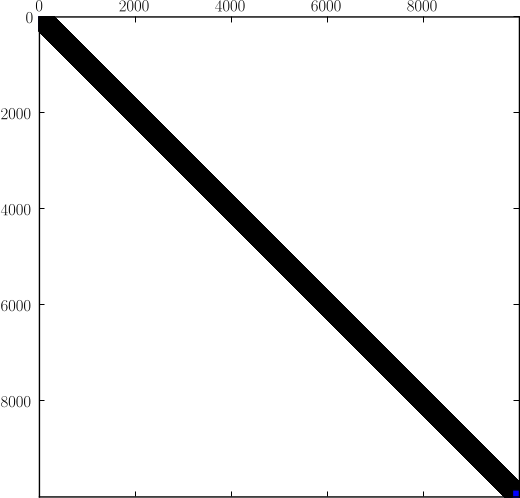
\includegraphics[width=.75\textwidth]{spy.png}
\caption{The output of the \li{spy()} command}
\label{fig:mpl_spy}
\end{figure}

%insert problem here that lets them play around with large sparse matrices in diff forms

\begin{comment}
\subsection*{Banded Matrices} % -----------------------------------------------

\begin{problem}
Write a function that takes an integer argument \li{n} and returns a full $n\times n$
tri-diagonal array with $2$'s along the diagonal and $-1$'s along
the two sub-diagonals above and below the diagonal.
\\(Hint: \li{np.diagflat()} may be useful.)

\label{full_tridiag}
\end{problem}
\end{comment}

\subsection*{Manipulating Sparse Matrices} % ----------------------------------

Scipy's \li{sparse} matrices behave a little differently than NumPy arrays.
You can multiply two sparse matrices element-wise with the \li{multiply()} method of one of the sparse matrices.

\begin{lstlisting}
>>> D = sparse.spdiags([2,3,4],0,3,3)
>>> C = sparse.spdiags(np.ones((3,3)), [-1,0,1], 3, 3)
>>> (D.multiply(C)).todense()
matrix([[ 2.,  0.,  0.],
        [ 0.,  3.,  0.],
        [ 0.,  0.,  4.]])
\end{lstlisting}

On the other hand, the asterisk \li{*} performs ordinary matrix multiplication.
You can also use the \li{dot} method of one of the sparse matrices.
However, you should NOT use \li{np.dot} on sparse matrices because it may return an incorrect answer.

\begin{lstlisting}
# One correct way to mutliply sparse matrices
>>> (D.dot(C)).todense()
matrix([[ 2.,  2.,  0.],
        [ 3.,  3.,  3.],
        [ 0.,  4.,  4.]])
\end{lstlisting}

Addition and scalar multiplication are implemented as usual.

\begin{lstlisting}
>>> (D + 3*C).todense()
matrix([[ 5.,  3.,  0.],
        [ 3.,  6.,  3.],
        [ 0.,  3.,  7.]])
\end{lstlisting}

\section*{Using Sparse Matrices to Reduce Runtimes} % =========================

In addition to spatial complexity, the \li{sparse} module can reduce temporal complexity.
Consider the linear system $A x = b$, where $A$ is a $100000\times 100000$ tri-diagonal matrix.
Storing a full matrix of that size requires 10 billion double-precision floating-point numbers.
Since it takes 8 bytes to store a double, we need roughly 80GB to store the full matrix.
Lack of storage space makes this system impossible to solve for most desktop computers, but even more problematic is the temporal complexity.
Methods for directly solving a linear system are usually $O(n^3)$.
As a result, even if the computer could store an 80GB matrix in RAM, it would still take several weeks to solve the system.
%However, since we don't typically have computers with that much available RAM, most of the
%matrix would have to be stored on the hard drive, so the computation would probably take between $6$ months to a year.

The point is, even as computers increase in processing speed and memory, we can still easily construct problems that they will struggle to solve in a reasonable amount of time.
However, if we store the tri-diagonal matrix as a \li{sparse} matrix, we can solve the linear system, even with a modest computer.

Let's first compute the spatial complexity of the above system when $A$ is stored as a sparse matrix.
There are three diagonals that have roughly $100000$ non-zero entries.
That's $300000$ double-precision floating point numbers, which is about 2.4 MB, or less storage than your favorite song.
Thus, the sparse matrix will easily fit into the computer's RAM. Furthermore, the temporal complexity for solving a tri-diagonal matrix is $O(n)$.
\footnote{Because there are fast algorithms for solving a tri-diagonal linear system, you may think that there are fast algorithms for inverting a tri-diagonal matrix.
In fact this is not true, and the inverse of a sparse matrix is usually not sparse.
There is rarely a good reason to invert a matrix, sparse or dense.}
Let's see how long it takes to solve the system when $A$ and $b$ are filled with random data.

\begin{lstlisting}
>>> from scipy.sparse import linalg as sl
>>> G = np.random.rand(3, 100000)
>>> b = np.random.rand(1, 100000)
>>> A = sparse.spdiags(G,[-1,0,1],100000,100000, format='csr')
>>> def solSys():
...     return sl.spsolve(A, b)

>>> %timeit solSys()
1 loops, best of 3: 80.8 ms per loop

\end{lstlisting}

This computer solved the system in only 80.8 milliseconds.

\begin{comment}
\begin{problem}
Write a function that accepts an integer argument \li{n} as well as a keyword argument \li{sparse} whose value is either \li{True} or \li{False} (default to \li{False}).
Then do the following:
\begin{enumerate}
\item Inside of the function, use your previous solutions to generate an $n \times n$ tri-diagonal array $A$ -- either sparse or full depending on the value of the \li{sparse} argument.
\item Generate an $n \times 1$ random array $b$
\item Solve the system $Ax = b$, using either \li{scipy.sparse.linalg.spsolve} or \li{scipy.linalg.solve}
(again depending on the value of \li{sparse}) and return the solution.
\item Time the function for \li{n = 2000} using both the sparse and the full option.
\end{enumerate}
\end{problem}
\end{comment}

\begin{problem}
Write a function that accepts an integer argument $n$ and does the following:
\begin{enumerate}
\item Generates an $n \times 1$ random array $b$.
\item Solves the linear system $Ax = b$, where $A$ is the tri-diagonal array in Problem \ref{prob:sparse_tridiag} of size $n \times n$.
\end{enumerate}
\end{problem}

\begin{problem}
Write a function that accepts an integer argument \li{n} and returns $\lambda n^2$, where
$\lambda$ is the smallest eigenvalue of the sparse tri-diagonal array you built in Problem \ref{prob:sparse_tridiag}.

If \li{A} is your tri-diagonal matrix, calculate $\lambda$ using the method \li{scipy.sparse.linalg.eigs} with the command \li{sl.eigs(A.asfptype(), which = 'SM')}.
The code \li{A.asfptype()} ensures that your matrix has the right data type, and the parameter \li{which = 'SM'} tells the function to look for the smallest eigenvalues.
This command will return several of the smallest eigenvalues of \li{A}, and you will have to select the smallest of these.
Read the documentation of \li{sl.eigs} for more information.

What value does $\lambda n^2$ approach as $n$ approaches infinity?
This value is meaningful in operator theory.
\li{Hint}: This value is the square of an important number.

\end{problem}

\newpage

\section*{Additional Material} % ==============================================

\subsection*{The Cholesky Decomposition} % ------------------------------------

The Cholesky decomposition requires half the calculations and memory of the LU decomposition.
Furthermore, it is \emph{numerically stable}, which means that round-off errors do not propagate throughout the computation.
Because of its efficiency and numerical stability, the Cholesky decomposition is used to solve least squares, optimization, and state estimation problems.

However, the Cholesky decomposition is only applicable to Hermitian positive definite matrices.
A matrix $A$ is positive definite if  $\mathbf{z}\trp A\mathbf{z} > 0$ for all $\mathbf{z} \neq 0$.
Furthermore, $A$ is Hermitian if $A = A^*$ where $A^* = \overline{A\trp }$, so a real Hermitian matrix is just a symmetric matrix.
The Cholesky decomposition is the matrix equivalent to taking the square root of a positive real number.

The Cholesky decomposition of a $A$ is a lower-triangular matrix $L$ such that

\begin{equation*}
 A = LL^*.
\end{equation*}

The entries of $L$ are calculated as follows.

\begin{align*}
&L_{i,j} = \frac{1}{L_{j,j}}\left(A_{i,j} -\sum_{k=1}^{j-1}{L_{i,k}L_{j,k}}\right) \mbox{ for $i>j$} \\ \\
&L_{i,i} = \sqrt{A_{i,i} - \sum_{k=1}^{i-1}{L_{i,k}L_{i,k}}}.
\end{align*}

Notice that the entries of $L$ are defined recursively, with dependencies as diagrammed in Figure \ref{fig:cholesky}.
Thus, an implementation of the Cholesky decomposition must compute the entries of $L$ in the correct order.

\begin{figure}
\begin{tikzpicture}[red dot/.style={draw, circle, fill=red, red},
    norm/.style={draw=none}, xscale=1.5, yscale=1.5]

\begin{scope}[shift={(4,0)}]
\draw [-,ultra thick](-.2,0)--(-.2,2.5);
\draw [-,ultra thick](2.7,0)--(2.7,2.5);
\draw [-,ultra thick](-.2,0)--(0,0);
\draw [-,ultra thick](-.2,2.5)--(0,2.5);
\draw [-,ultra thick](2.7,2.5)--(2.5,2.5);
\draw [-,ultra thick](2.7,0)--(2.5,0);

\node[norm,black](bk1)at(.25,2.25){\LARGE \textbullet};
\node[norm,black](bk2)at(.75,1.75){\LARGE \textbullet};
\node[norm,black!25!](b1)at(1.25,1.25){\LARGE \textbullet};
\node[norm,black](bk3)at(1.75,.75){\LARGE \textbullet};
\node[norm, black](bk4)at(2.25,.25){\LARGE \textbullet};
\node[norm, black!25!](b2)at(.25,1.25){\LARGE \textbullet};
\node[norm,black!25!](b3)at(.75,1.25){\LARGE \textbullet};
\node[norm,black!25!](b4)at(.25,.25){\LARGE \textbullet};
\node[norm,black!25!](b3)at(.75,.25){\LARGE \textbullet};
\node[norm, shadecolor](r1)at(1.25,.25){\Huge \textbullet};

\end{scope}

\begin{scope}
\draw [-,ultra thick](-.2,0)--(-.2,2.5);
\draw [-,ultra thick](2.7,0)--(2.7,2.5);
\draw [-,ultra thick](-.2,0)--(0,0);
\draw [-,ultra thick](-.2,2.5)--(0,2.5);
\draw [-,ultra thick](2.7,2.5)--(2.5,2.5);
\draw [-,ultra thick](2.7,0)--(2.5,0);


\node[norm, shadecolor](r1)at(1.75,.75){\Huge \textbullet};
\node[norm,black](bk1)at(.25,2.25){\LARGE \textbullet};
\node[norm,black](bk2)at(1.25,1.25){\LARGE \textbullet};
\node[norm,black](bk3)at(.75,1.75){\LARGE \textbullet};
\node[norm,black](bk4)at(2.25,.25){\LARGE \textbullet};
\node[norm,black!25!](bk1)at(.25,.75){\LARGE \textbullet};
\node[norm,black!25!](bk1)at(.75,.75){\LARGE \textbullet};
\node[norm, black!25!](bk1)at(1.25,.75){\LARGE \textbullet};
\end{scope}
\end{tikzpicture}
\label{fig:cholesky}
\caption{The entries of $L$ in the Cholesky decomposition are defined recursively, as illustrated in this picture.
To calculate the green entry, you need to know each of the light gray entries.}
\end{figure}


\begin{problem}
Write a function that finds the Cholesky decomposition of a Hermitian positive definite matrix.
Hint: To generate symmetric positive definite matrices on which to test your function, recall that for any matrix $A$, the matrix $A\trp A$ is symmetric and positive definite.
\end{problem}

The \li{linalg} module of SciPy includes an optimized Cholesky decomposition.
As with the LU decomposition, SciPy has the methods \li{la.cho_factor} and \li{la.cho_solve}.

\begin{problem}
Repeat problem \ref{prob:solve}, this time using the methods \li{la.cho_factor} and \li{la.cho_solve}.
\end{problem}
